\documentclass[12pt]{article}
	
\title{CSC 320 - Worksheet 5}
\author{Nadeem Abdul Hamid}
\date{January 25, 2024}  


\usepackage[margin=1in]{geometry}		% For setting margins
\usepackage{amsmath}				% For Math
\usepackage{amsthm}
\usepackage{fancyhdr}				% For fancy header/footer
\usepackage{graphicx}				% For including figure/image
\usepackage{cancel}					% To use the slash to cancel out stuff in work
\usepackage[shortlabels]{enumitem}
\usepackage{hyperref}
\usepackage{jigsaw}

\usepackage{algorithm,caption}
\usepackage{algpseudocodex}
% docs: https://ctan.math.washington.edu/tex-archive/macros/latex/contrib/algpseudocodex/algpseudocodex.pdf


%%%%%%%%%%%%%%%%%%%%%%
% Set up fancy header/footer
% taken from https://www.overleaf.com/latex/templates/homework-template/yvgnmrbywwnp
\makeatletter    % for \@ in \@title
\pagestyle{fancy}
\fancyhead[LO,L]{\@author}
\fancyhead[CO,C]{\@title}
\fancyhead[RO,R]{\@date}
\fancyfoot[LO,L]{}
\fancyfoot[CO,C]{\thepage}
\fancyfoot[RO,R]{}
\renewcommand{\headrulewidth}{0.4pt}
\renewcommand{\footrulewidth}{0.4pt}
\makeatother    % restore
%%%%%%%%%%%%%%%%%%%%%%


%%%%%%%%%%%%%%%%%%%%%%
% from: https://tex.stackexchange.com/questions/14667/does-latex-define-a-semantic-equivalent-of-textbf
\makeatletter
\newcommand{\strong}[1]{\@strong{#1}}
\newcommand{\@@strong}[1]{\textbf{\let\@strong\@@@strong#1}}
\newcommand{\@@@strong}[1]{\textnormal{\let\@strong\@@strong#1}}
\let\@strong\@@strong
\makeatother
%%%%%%%%%%%%%%%%%%%%%%


\newcommand{\emptybox}[2][\textwidth]{%
  \begingroup
  \setlength{\fboxsep}{-\fboxrule}%
  \noindent\framebox[#1]{\rule{0pt}{#2}}%
  \endgroup
}

\newtheorem{theorem}{Theorem}
\newtheorem{lemma}{Lemma}


\begin{document}

\section{Backtracking}

\subsection{Text Segmentation}

From page 83-84:

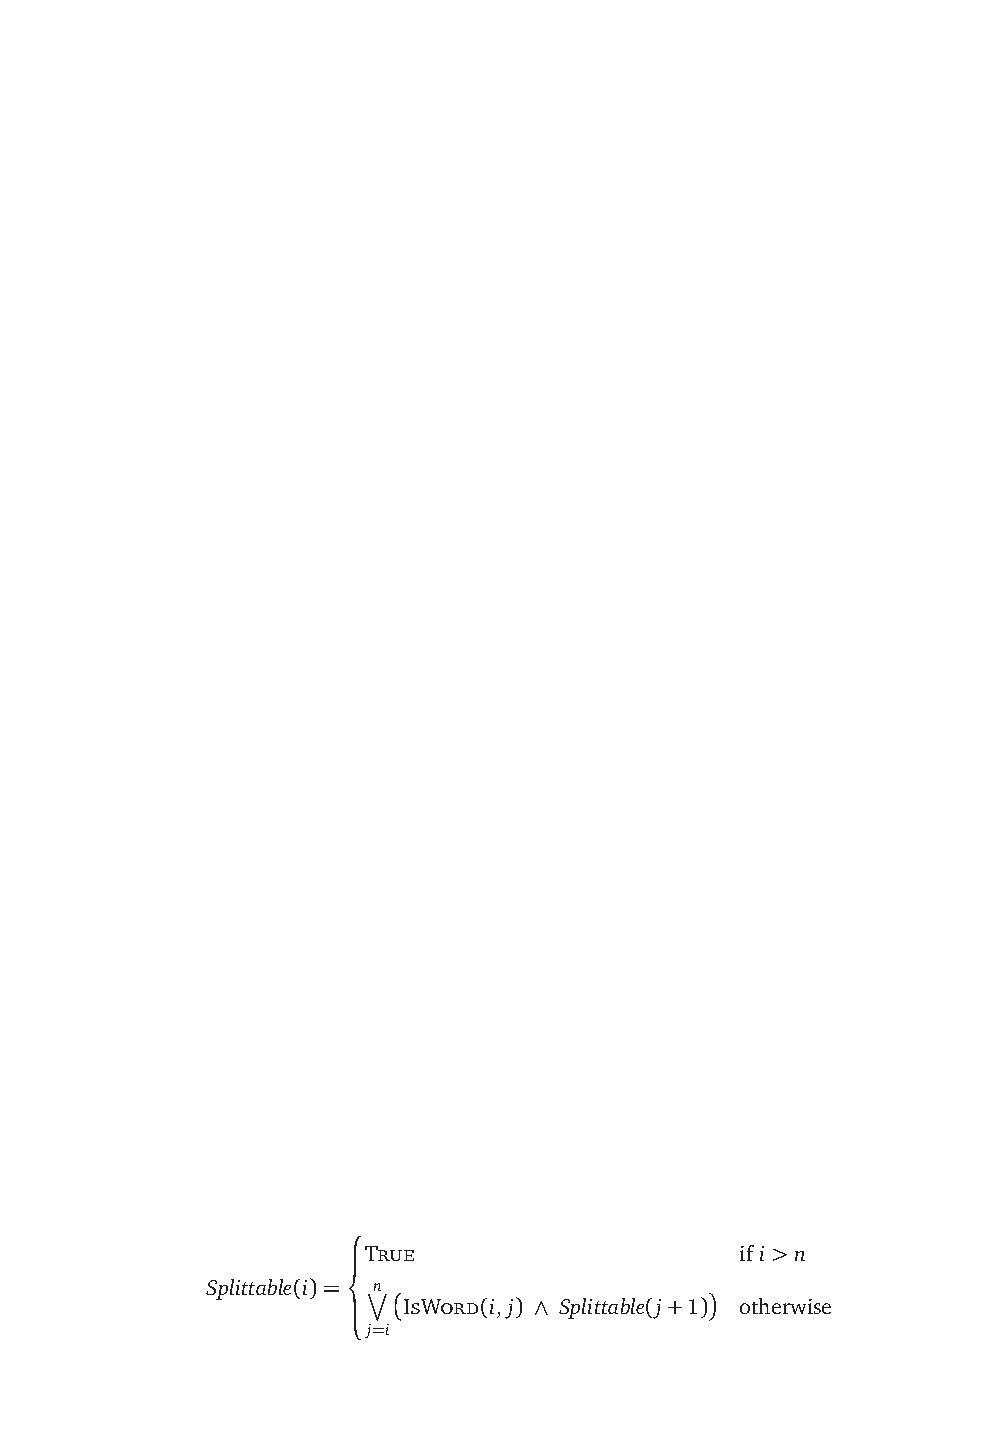
\includegraphics{w05-splittable.pdf}
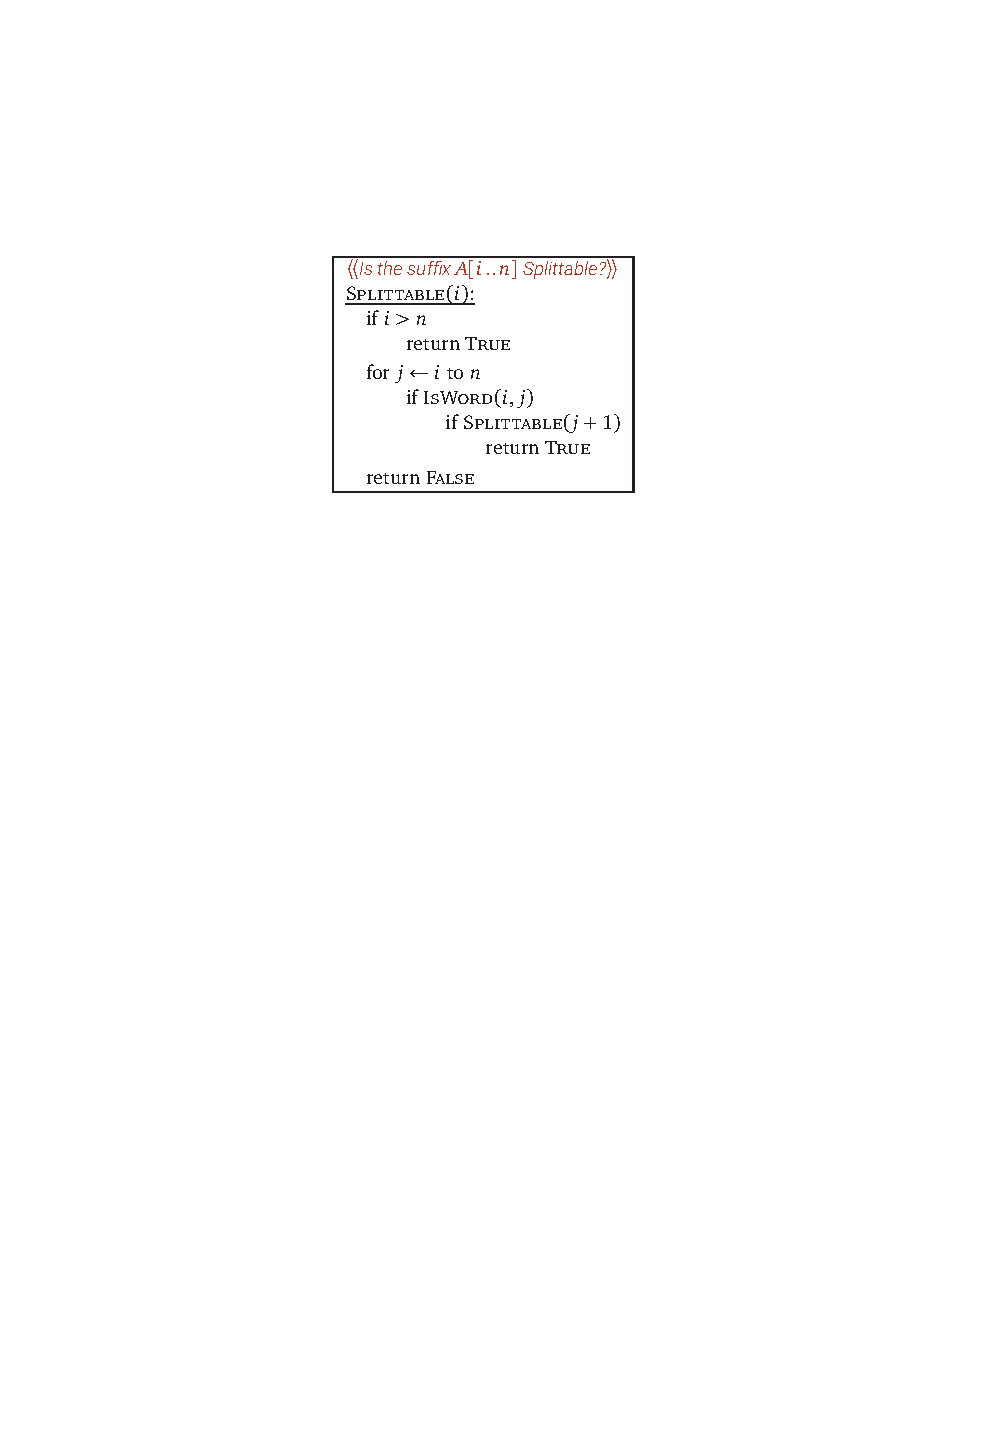
\includegraphics{w05-splittable-pc.pdf}

Suppose \textsc{IsWord} is defined as:

\[
\textsc{IsWord}(i,j) := (A[i..j] = \textrm{reverse}(A[i..j]))
\]

\begin{itemize}
  \item Trace $Splittable(1)$ on the array, $A[1..9] = \texttt{"AABCCBAAZ"}$.
  \vspace{2in}
  \item Suppose we want to know the \emph{minimum number of splits} needs to split $A[1..n]$ into valid ``words'' (according to \textsc{IsWord}). Let $MinSplits(i)$ be a function that computes the minimal number of splits needed to split $A[i..n]$ into valid ``words''. Define $MinSplits(i)$.
\end{itemize}

\clearpage

\section{Subset Sum}

The \textsc{SubsetSum} problem: Given an array $A[1..n]$ of positive integers and a \emph{target} integer $T$, is there a subset of the elements of $A$ that add up to $T$?\\~

\begin{minipage}{1.0\textwidth}\centering
  \begin{tabular}{|*{8}{c|}}
      \hline
      5 & 6 & 3 & 6 & 5 & 2 & 8 & 10 \\
      \hline
    \end{tabular}
  \end{minipage}%


\begin{itemize}
  \item $T = 30$ ? 
  \item $T = 100$ ?
  
  \item Write an English description of what you want to calculate. (Work backwards from $A[n]$. Decide whether to include it or not, \ldots)
  \vspace{1in}
  \item Write a recursive definition of \textsc{SubsetSum}().
  \vspace{2in}
  \item Give a couple sentences (in English) of why your recurrence should work.
  \vspace{2in}
\end{itemize}


\clearpage

\section{Longest Increasing Subsequence}

Given an integer array $A[1..n]$, compute the length of the longest possible sequence of indices (not necessarily contiguous), $1 \leq i_1 < i_2 < \ldots < i_l \leq n$, such that $A[i_k] < A[i_{k+1}]$ for all $1 \leq k < l$.

Example:

\begin{minipage}{1.0\textwidth}\centering
  \begin{tabular}{|*{8}{c|}}
      \hline
      5 & -6 & 3 & 6 & -5 & 2 & 8 & 10 \\
      \hline
    \end{tabular}
  \end{minipage}%

\begin{itemize}
  \item What is the optimal value for the array above? 
  \vspace*{.75in}
  \item Develop a recursive algorithm going left-to-right through the array, thinking ``do I include this element or not?'' for each element. (Will need to keep track of previously largest element.)
  \vspace{3in}
  \item Time complexity?
\end{itemize}

\clearpage
Alternate way of thinking about \textsc{LIS}: Ask ``What's the longest subsequence starting from me?'. 
\begin{itemize}
  \item Let $LISStart(i)$ be the length of the longest increasing subsequence
  among indices $i .. n$ that starts at index $i$. Develop a recurrence.
\end{itemize}

\end{document}



